\documentclass[a4paper,11pt,fleqn]{scrartcl}
\usepackage[german,ngerman]{babel}
\usepackage[utf8]{inputenc}
\usepackage[T1]{fontenc}
\usepackage[top=1.3in, bottom=1.2in, left=0.9in, right=0.9in]{geometry}
\usepackage{lmodern}
\usepackage{amssymb}
\usepackage{amsmath}
\usepackage{enumerate}
\usepackage{fancyhdr}
\usepackage{color}
\usepackage{pgfplots}
\usepackage{tikz}

% ------------------------------------------------------

% Commands

\newcommand{\todo}{\textcolor{red}{\textbf{TODO}}}
\newcommand{\authorinfo}{Arne Struck, Jonathan Werner}
\newcommand{\titleinfo}{HLR OPENMP, Blatt 4}
\newcommand{\qed}{\ \square}


% ------------------------------------------------------

% Title & Pages

\title{\titleinfo}
\author{\authorinfo}

\pagestyle{fancy}
\fancyhf{}
\fancyhead[L]{\authorinfo}
\fancyhead[R]{\titleinfo}
\fancyfoot[C]{\thepage}

\begin{document}
\maketitle
\notag


\section{Optimierung}\label{optimierung}

\textbf{Sequentiell, ohne \texttt{-fopenmp}:}

\texttt{./partdiff-seq 1 2 512 2 2 200} braucht \textbf{120.29s}.

\textbf{1 Thread, mit \texttt{-fopenmp}:}

\texttt{./partdiff-seq 1 2 512 2 2 200} braucht \textbf{120.65s}.

\textbf{12 Threads, mit \texttt{-fopenmp}:}

\texttt{./partdiff-seq 1 2 512 2 2 200} braucht \textbf{14.9s}.

\textbf{Mit verschiedenen Schedulings, jw 12 Threads:}

\begin{itemize}
\itemsep1pt\parskip0pt\parsep0pt
\item
  \textbf{\texttt{schedule(dynamic, 1)}:}

  \begin{itemize}
  \itemsep1pt\parskip0pt\parsep0pt
  \item
    \texttt{./partdiff-seq 1 2 512 2 2 200} braucht \textbf{11.39s}.
  \item
    Speedup zu ohne OMP: \textbf{10.59}. The winner! :)
  \end{itemize}
\item
  \textbf{\texttt{schedule(dynamic, 4)}:}

  \begin{itemize}
  \itemsep1pt\parskip0pt\parsep0pt
  \item
    \texttt{./partdiff-seq 1 2 512 2 2 200} braucht \textbf{14.2s}.
  \item
    Speedup zu ohne OMP: \textbf{\textasciitilde{}8.5}.
  \end{itemize}
\item
  \textbf{\texttt{schedule(guided)}:}

  \begin{itemize}
  \itemsep1pt\parskip0pt\parsep0pt
  \item
    \texttt{./partdiff-seq 1 2 512 2 2 200} braucht \textbf{12.3s}.
  \item
    Speedup zu ohne OMP: \textbf{9.8}.
  \end{itemize}
\item
  \textbf{\texttt{schedule(static, 1)}:}

  \begin{itemize}
  \itemsep1pt\parskip0pt\parsep0pt
  \item
    \texttt{./partdiff-seq 1 2 512 2 2 200} braucht \textbf{14.1s}.
  \end{itemize}
\item
  \textbf{\texttt{schedule(static, 2)}:}

  \begin{itemize}
  \itemsep1pt\parskip0pt\parsep0pt
  \item
    \texttt{./partdiff-seq 1 2 512 2 2 200} braucht \textbf{14.7s}.
  \end{itemize}
\item
  \textbf{\texttt{schedule(static, 16)}:}

  \begin{itemize}
  \itemsep1pt\parskip0pt\parsep0pt
  \item
    \texttt{./partdiff-seq 1 2 512 2 2 200} braucht \textbf{14.57s}.
  \end{itemize}
\end{itemize}

Zeit benötigt: 2h. Fehlersuche? Ja, zuerst haben wir die simple
interference function geenommen und dadurch nur ein Speedup von 4
erreicht.


\newpage
\section{Messungen}\label{messungen}

\subsection{Messung 1}\label{messung-1}
\begin{center}
\begin{tabular}[c]{l|l|l}
procs & speedup & time in sec \\ \hline

1 (no OMP) & 1 & 120.29 \\
1 & 1 & 120.65 \\
2 & 2.044222298 & 59.02 \\
3 & 2.960009814 & 40.76 \\
4 & 4.045942321 & 29.82 \\
5 & 4.868845843 & 24.78 \\ 
6 & 5.952146029 & 20.27 \\
7 & 6.710233593 & 17.98 \\
8 & 7.65060241 & 15.77 \\
9 & 8.431167016 & 14.31 \\
10 & 9.1332324 & 13.21 \\
11 & 9.913722268 & 12.17 \\
12 & 9.995857498 & 12.07 \\
\end{tabular}
\end{center}

\begin{figure}[htbp]
\centering
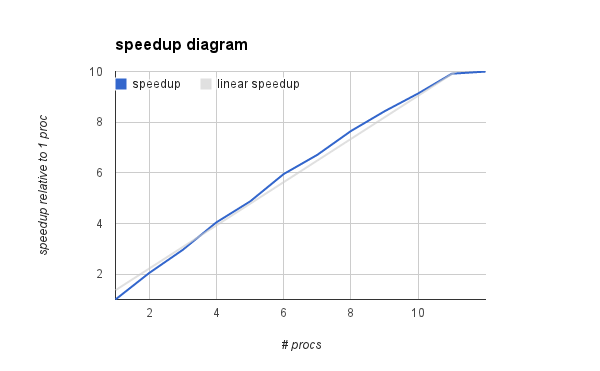
\includegraphics[scale=0.8]{speedup.png}
\caption{}
\end{figure}

Der Speedup des Programmes ist zu Anfang Linear (scheinbare Superlinearität ist auf messungenauigkeiten zurückzuführen). Dies deckt sich mit dem Amdahlschen Gesetz. Das Resultat deckt sich also mit den Erwartungen an ein gut zu parallelisierendes Programm. Um weitere Aussagen treffen zu können, müsste die Thread-Anzahl drastisch erhöht werden. Leider stößt Open-MP hier an seine Grenzen, zu mindest in Zusammenspiel mit der uns zur Verfügung stehenden Architektur.

\subsection{Messung 2}
\begin{tikzpicture}
    \begin{axis}[
        xmode = log,
        ymode = log,
        height = 10cm,
        width = 14cm,        
        xlabel= \text{interline count},
        ylabel= \text{time in s}
    ]
    \axispath\draw
            (7.49165,-10.02171)
        |-  (8.31801,-11.32467)
        node[near start,left] {$\frac{dy}{dx} = -1.58$};
      \addplot[smooth, mark=*, blue] plot coordinates {
        (1, 0.09)
		(2, 0.11)
		(4, 0.2)
		(8, 0.37)
		(16, 1)
		(32, 3.4)
		(64, 12.59)
		(128, 48.4)
		(256, 194)
		(512, 760)
    };
    \end{axis}
\end{tikzpicture}
 \\ \\
\begin{center}
Verwendete Werte: \\ \quad \\
	\begin{tabular}[c]{l|l}
	interlines & time \\ \hline
	1& 0.09 \\
	2& 0.11 \\
	4& 0.2 \\
	8& 0.37 \\
	16& 1 \\
	32& 3.4 \\
	64& 12.59 \\
	128& 48.4 \\
	256& 194 \\
	512& 760 \\
\end{tabular}
\end{center}

Die benötigte Zeit nimmt mit der Erhöhung der Interlinegröße zu. Diese Zunahme sollte aufgrund des Aufbaus der Matrix quadratisch-exponentiell zunehmen, da beide Dimensionen mit den Interlines um die selbe Größe wachsen. Da allerdings die Berechnung auf 12 threads aufgeteilt werden, ist nur ein Zwölftel der Zeit des rein sequentiellen Ansatzes theoretisch nötig. Diese Vermutung wird durch unsere Tests nur partiell getützt. Zu Anfang folgt die zeitliche Zunahme ungefähr diesem Muster, bei dem Übergang von 256 auf 512 Interlines nimmt die benötigte Zeit leider über die Maßen zu. Dies liegt vermutlich sowohl daran, dass die Parallelisierung nicht perfekt ist, als auch an der Tatsache dass auch Open-MP keine perfekten Parallelisierungen schafft.

\end{document}
